% (find-LATEX "2021-2-C3-notacao-de-fisicos.tex")
% (defun c () (interactive) (find-LATEXsh "lualatex -record 2021-2-C3-notacao-de-fisicos.tex" :end))
% (defun C () (interactive) (find-LATEXsh "lualatex 2021-2-C3-notacao-de-fisicos.tex" "Success!!!"))
% (defun D () (interactive) (find-pdf-page      "~/LATEX/2021-2-C3-notacao-de-fisicos.pdf"))
% (defun d () (interactive) (find-pdftools-page "~/LATEX/2021-2-C3-notacao-de-fisicos.pdf"))
% (defun e () (interactive) (find-LATEX "2021-2-C3-notacao-de-fisicos.tex"))
% (defun o () (interactive) (find-LATEX "2021-1-C3-notacao-de-fisicos.tex"))
% (defun u () (interactive) (find-latex-upload-links "2021-2-C3-notacao-de-fisicos"))
% (defun v () (interactive) (find-2a '(e) '(d)))
% (defun d0 () (interactive) (find-ebuffer "2021-2-C3-notacao-de-fisicos.pdf"))
% (defun cv () (interactive) (C) (ee-kill-this-buffer) (v) (g))
%          (code-eec-LATEX "2021-2-C3-notacao-de-fisicos")
% (find-pdf-page   "~/LATEX/2021-2-C3-notacao-de-fisicos.pdf")
% (find-sh0 "cp -v  ~/LATEX/2021-2-C3-notacao-de-fisicos.pdf /tmp/")
% (find-sh0 "cp -v  ~/LATEX/2021-2-C3-notacao-de-fisicos.pdf /tmp/pen/")
%     (find-xournalpp "/tmp/2021-2-C3-notacao-de-fisicos.pdf")
%   file:///home/edrx/LATEX/2021-2-C3-notacao-de-fisicos.pdf
%               file:///tmp/2021-2-C3-notacao-de-fisicos.pdf
%           file:///tmp/pen/2021-2-C3-notacao-de-fisicos.pdf
% http://angg.twu.net/LATEX/2021-2-C3-notacao-de-fisicos.pdf
% (find-LATEX "2019.mk")
% (find-CN-aula-links "2021-2-C3-notacao-de-fisicos" "3" "c3m212nf" "c3nf")

% «.defs»	(to "defs")
% «.title»	(to "title")
%
% «.introducao»			(to "introducao")
% «.links»			(to "links")
% «.silvanus-thompson»		(to "silvanus-thompson")
% «.primeiro-exemplo»		(to "primeiro-exemplo")
% «.omitir-nomes»		(to "omitir-nomes")
% «.omitir-nomes-2»		(to "omitir-nomes-2")
% «.omitir-nomes-3»		(to "omitir-nomes-3")
% «.exercicio-1»		(to "exercicio-1")
% «.exercicio-1-dica»		(to "exercicio-1-dica")
% «.lendo-o-ST»			(to "lendo-o-ST")
% «.silvanus-triangle»		(to "silvanus-triangle")
% «.silvanus-escada»		(to "silvanus-escada")
% «.escada-contas»		(to "escada-contas")
% «.exercicio-2»		(to "exercicio-2")
% «.exercicio-2-dicas-2»	(to "exercicio-2-dicas-2")
% «.variaveis-novas»		(to "variaveis-novas")
% «.derivadas-parciais»		(to "derivadas-parciais")
% «.derivadas-parciais-th»	(to "derivadas-parciais-th")
% «.derivadas-parciais-e-ts»	(to "derivadas-parciais-e-ts")
% «.exercicio-7»		(to "exercicio-7")
% «.exercicio-8»		(to "exercicio-8")
%
% «.exercicio-2»		(to "exercicio-2")
% «.quadraticas-exemplos»	(to "quadraticas-exemplos")
% «.thomas»			(to "thomas")
% «.bortolossi»			(to "bortolossi")
% «.segundo-exemplo»		(to "segundo-exemplo")
%
% «.djvuize»	(to "djvuize")



% <videos>
% Video (not yet):
% (find-ssr-links     "c3m212nf" "2021-2-C3-notacao-de-fisicos")
% (code-eevvideo      "c3m212nf" "2021-2-C3-notacao-de-fisicos")
% (code-eevlinksvideo "c3m212nf" "2021-2-C3-notacao-de-fisicos")
% (find-c3m212nfvideo "0:00")

\documentclass[oneside,12pt]{article}
\usepackage[colorlinks,citecolor=DarkRed,urlcolor=DarkRed]{hyperref} % (find-es "tex" "hyperref")
\usepackage{amsmath}
\usepackage{amsfonts}
\usepackage{amssymb}
\usepackage{pict2e}
\usepackage[x11names,svgnames]{xcolor} % (find-es "tex" "xcolor")
\usepackage{colorweb}                  % (find-es "tex" "colorweb")
%\usepackage{tikz}
%
% (find-dn6 "preamble6.lua" "preamble0")
%\usepackage{proof}   % For derivation trees ("%:" lines)
%\input diagxy        % For 2D diagrams ("%D" lines)
%\xyoption{curve}     % For the ".curve=" feature in 2D diagrams
%
\usepackage{edrx21}               % (find-LATEX "edrx21.sty")
\input edrxaccents.tex            % (find-LATEX "edrxaccents.tex")
\input edrx21chars.tex            % (find-LATEX "edrx21chars.tex")
\input edrxheadfoot.tex           % (find-LATEX "edrxheadfoot.tex")
\input edrxgac2.tex               % (find-LATEX "edrxgac2.tex")
%
%\usepackage[backend=biber,
%   style=alphabetic]{biblatex}            % (find-es "tex" "biber")
%\addbibresource{catsem-slides.bib}        % (find-LATEX "catsem-slides.bib")
%
% (find-es "tex" "geometry")
\usepackage[a6paper, landscape,
            top=1.5cm, bottom=.25cm, left=1cm, right=1cm, includefoot
           ]{geometry}
%
\begin{document}

\catcode`\^^J=10
\directlua{dofile "dednat6load.lua"}  % (find-LATEX "dednat6load.lua")

%L dofile "edrxtikz.lua"  -- (find-LATEX "edrxtikz.lua")
%L dofile "edrxpict.lua"  -- (find-LATEX "edrxpict.lua")
%L dofile "2021-1-C3-3D.lua" -- (find-LATEX "2021-1-C3-3D.lua")
%L
%L V3.__index.tostring = function (v) return v:v2string() end
\pu

% «defs»  (to ".defs")
% (find-LATEX "edrx21defs.tex" "colors")
% (find-LATEX "edrx21.sty")

\def\pictgray#1{{\color{GrayPale}\linethickness{0.3pt}#1}}

\def\u#1{\par{\footnotesize \url{#1}}}

\def\asf#1{〈\textsf{#1}〉}

\def\drafturl{http://angg.twu.net/LATEX/2021-2-C3.pdf}
\def\drafturl{http://angg.twu.net/2021.2-C3.html}
\def\draftfooter{\tiny \href{\drafturl}{\jobname{}} \ColorBrown{\shorttoday{} \hours}}



%  _____ _ _   _                               
% |_   _(_) |_| | ___   _ __   __ _  __ _  ___ 
%   | | | | __| |/ _ \ | '_ \ / _` |/ _` |/ _ \
%   | | | | |_| |  __/ | |_) | (_| | (_| |  __/
%   |_| |_|\__|_|\___| | .__/ \__,_|\__, |\___|
%                      |_|          |___/      
%
% «title»  (to ".title")
% (c3m212nfp 1 "title")
% (c3m212nfa   "title")

\thispagestyle{empty}

\begin{center}

\vspace*{1.2cm}

{\bf \Large Cálculo 3 - 2021.2}

\bsk

Aula 11: ``notação de físicos''

\bsk

Eduardo Ochs - RCN/PURO/UFF

\url{http://angg.twu.net/2021.2-C3.html}

\end{center}

\newpage

%  _   _ _____ 
% | \ | |  ___|
% |  \| | |_   
% | |\  |  _|  
% |_| \_|_|    
%              
% «intro-nf»  (to ".intro-nf")
% (c3m212typesp 9 "intro-nf")
% (c3m212typesa   "intro-nf")

{\bf Introdução à ``notação de físicos''}

\ssk


\scalebox{0.7}{\def\colwidth{7cm}\firstcol{

Nós vamos aprender a usar duas convenções de notação matemática no
curso -- ou, pra encurtar, duas ``notações''. O Bortolossi usa uma
notação muito mais precisa, que eu vou chamar de ``notação de
matemáticos'', e o Silvanus Thompson usa uma notação mais intuitiva
mas bem mais difícil de formalizar, que eu vou chamar de ``notação de
físicos''.

\ssk

Na ``notação de físicos'' muitos símbolos vão ser {\sl abreviações} e
as regras pra expandir essas abreviações vão depender do contexto. Vão
existir algumas convenções pra expandir essas abreviações que vão ser
seguidas {\sl quase} sempre, mas vão existir muitas exceções -- e
muitos casos ambíguos...

% «introducao»  (to ".introducao")
% (c3m211nfp 2 "introducao")
% (c3m211nfa   "introducao")

}\anothercol{

% (find-bortolossi5page (+ -162 164) "5.2. Definições e exemplos")
% (find-bortolossi5page (+ -162 165)   "Fig. 5.2: Interpretação geométrica")
% (find-bortolossi5page (+ -162 167)   "Exemplo 5.1: Cobb-Douglas")
% (find-bortolossi5page (+ -162 170)   "derivada parcial")
% (find-bortolossi5page (+ -162 171)   "a notação D_1 f é a mais clara")
% (find-bortolossi5page (+ -162 172)   "omitir os pontos onde as parciais são calculadas")

Na página 170--172 do cap.5 o Bortolossi fala de algumas convenções
sobre variáveis que ele vai usar o mínimo possível, porque elas às
vezes são difíceis de interpretar e às vezes são ambíguas...

Isso é um assunto bem maior e mais complicado do que parece. Quando eu
fiz graduação em algumas matérias essas convenções -- que eu vou
chamar de ``notação de físicos'' -- eram totalmente
\ColorRed{proibidas}, mas em outras elas eram tratadas como algo
\ColorRed{óbvio} que \ColorRed{todo mundo sabia usar}.

A gente vai aprender alguns dos princípios por trás da ``notação de
físicos'' e vamos como usar essa ``notação de físicos'' como uma
\ColorRed{abreviação} pra uma notação muito menos ambígua que
matemáticos ``estritos'' aceitam.

}}



\newpage

%  __  __       _     ____   ___ ____  _   _ 
% |  \/  | __ _| |_  |___ \ / _ \___ \/ | / |
% | |\/| |/ _` | __|   __) | | | |__) | | | |
% | |  | | (_| | |_   / __/| |_| / __/| |_| |
% |_|  |_|\__,_|\__| |_____|\___/_____|_(_)_|
%                                            
% «material-de-2021.1»  (to ".material-de-2021.1")
% (c3m212typesp 8 "material-de-2021.1")
% (c3m212typesa   "material-de-2021.1")

{\bf Material do semestre passado}


\scalebox{0.45}{\def\colwidth{10cm}\firstcol{

    No semestre passado eu usei a ``notação de físicos'' pela primeira
    vez no curso de Cálculo 3, e dei uma parte do curso alternando
    entre três livros: o do Bortolossi (``notação de matemáticos''), o
    do Silvanus Thompson (``notação de físicos''), e o do Thomas (que
    usa as duas notações). Desta vez eu vou fazer a mesma coisa, só
    que de um jeito mais organizado que o do semestre passado, porque:
    1) eu vou reusar bastante material do semestre passado, 2) agora
    que eu acho que sei ``todas'' as regras necessárias pra traduzir a
    ``notação de físicos'' pra ``notação de matemáticos''... obs: esse
    ``agora eu acho que sei todas as regras'' quer dizer ``agora eu
    tenho um conjunto de regras de tradução que {\sl parece} ser
    suficiente pra traduzir {\sl tudo que a gente vai usar} da
    `notação de físicos' em Cálculo 3 pra `notação de
    matemáticos'\,''. Ninguém que eu conheço sabe fazer essa tradução
    formalmente, e eu estou conversando de vez em quando com umas
    pessoas de outras universidades pra ver se elas concordam com a
    minha tradução...

  }\def\colwidth{13cm}\anothercol{

    Aqui tem uma lista -- ainda bem incompleta -- de PDFs e vídeos do
    semestre passado sobre ``notação de físicos'':

    \bsk
    
    % (c3m211nfp 1 "title")
    % (c3m211nfa   "title")
    % (c3m211nfa   "title" "Aula 14: Notação de físicos")
    Aula 14: Notação de físicos
    \u{http://angg.twu.net/LATEX/2021-1-C3-notacao-de-fisicos.pdf}

    \bsk

    % (c3m211nfa "video-1")
    % (find-c3m211nfvideo "0:00" "30/jul/2021: introdução à NF, versão preliminar")
    30/jul/2021: introdução à NF, versão preliminar:
    \u{http://angg.twu.net/eev-videos/2021-1-C3-notacao-de-fisicos.mp4}
    \u{https://www.youtube.com/watch?v=fMNgr5wDMek}

    \bsk

    % (c3m211nfa "video-2")
    % (find-c3m211nf2video "0:00" "4/ago/2021: Segundo vídeo sobre notação de físicos")
    4/ago/2021: Segundo vídeo sobre notação de físicos
    \u{http://angg.twu.net/eev-videos/2021-1-C3-notacao-de-fisicos-2.mp4}
    \u{https://www.youtube.com/watch?v=bjBlOqO-7Do}

    \bsk

    % (c3m211nfa "video-3")
    % (find-c3m211nfstrvideo "0:00" "6/ago/2021: Silvanus Thompson: triângulo")
    6/ago/2021: Silvanus Thompson: triângulo
    \u{http://angg.twu.net/eev-videos/2021-1-C3-notacao-de-fisicos-s-tr.mp4}
    \u{https://www.youtube.com/watch?v=hOWVxOgv9p0}

    \bsk

    % (c3m211nfa "video-4")
    % (find-c3m211nfsescvideo "0:00" "6/ago/2021: Silvanus Thompson: o exemplo da escada")
    6/ago/2021: Silvanus Thompson: o exemplo da escada
    \u{http://angg.twu.net/eev-videos/2021-1-C3-notacao-de-fisicos-s-esc.mp4}
    \u{https://www.youtube.com/watch?v=-0QxJty23hQ}

    \bsk

    % (c3m211qa "video-4")
    % (find-c3m211q4video "0:00" "20/ago/2021 - Thompson/Gardner")
    20/ago/2021 - Thompson/Gardner
    \u{http://angg.twu.net/eev-videos/2021-1-C3-funcoes-quadraticas-4.mp4}
    \u{https://www.youtube.com/watch?v=d0fnURoPI9Q}



}}


\newpage

% «silvanus-thompson»  (to ".silvanus-thompson")
% (c3m212nfp 4 "silvanus-thompson")
% (c3m212nfa   "silvanus-thompson")
% (c3m211nfp 3 "silvanus-thompson")
% (c3m211nfa   "silvanus-thompson")
% (find-books "__analysis/__analysis.el" "thompson")

{\bf Silvanus P.~Thompson: Calculus Made Easy (1910)}

Vou usar bastante o livro do Silvanus P.~Thompson...

Ele está em inglês, mas descobri uma versão em \LaTeX{} dele 

feita a partir de uma versão em domínio público --- esta aqui:

\ssk

{\footnotesize

\url{https://www.gutenberg.org/files/33283/33283-pdf.pdf}

}

\ssk

que eu consigo modificar. Vou tentar traduzir algumas

páginas dessa versão pra português.

\msk

Links pra uma versão em HTML do livro

e pra comentários sobre ela:

\ssk

{\footnotesize

\url{https://calculusmadeeasy.org/}

\url{https://avidemia.com/calculus-made-easy/}

\url{https://news.ycombinator.com/item?id=27991120}

\url{https://news.ycombinator.com/from?site=calculusmadeeasy.org}

}

\bsk

\standout{Obs:} o Silvanus não distingue $dx$ de $Δx$.


\newpage

% «primeiro-exemplo»  (to ".primeiro-exemplo")
% (c3m212typesp 10 "primeiro-exemplo")
% (c3m212typesa    "primeiro-exemplo")
% (c3m211nfp 6 "primeiro-exemplo")
% (c3m211nfa   "primeiro-exemplo")

{\bf Um primeiro exemplo}

Digamos que $y=\sqrt{x}$.

Podemos considerar que $x$ e $y$ ``variam juntos'',

``obedecendo certas restrições''. O conjunto dos pontos $(x,y)$

que obedecem essas restrições é $\setofxyst{y = \sqrt{x}}$

e o gráfico é:
%
% (find-latexscan-links "C3" "20210804_sqrt")
% (find-xpdf-page "~/LATEX/2021-1-C3/20210804_sqrt.pdf")
$$\myvcenter{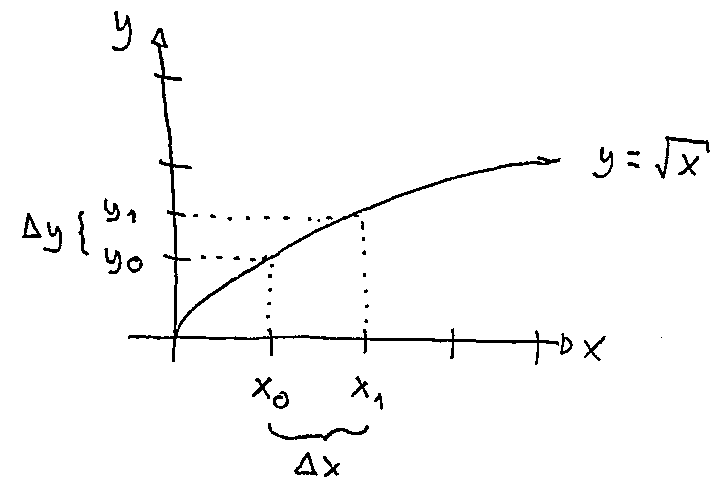
\includegraphics[height=4cm]{2021-1-C3/20210804_sqrt.pdf}}
  \qquad
  \begin{array}{rcl}
    x_0,x_1&∈&\R \\ 
    y_0 &=& \sqrt{x_0} \\ 
    y_1 &=& \sqrt{x_1} \\ 
    Δx &=& x_1 - x_0 \\
    Δy &=& y_1 - y_0 \\
    \\
  \end{array}
$$


\newpage

{\bf Um primeiro exemplo (2)}

Em geral vamos considerar que $x_0$ é ``mais fixo'' do que $x_1$.

Quando dizemos ``diminua $Δx$; ele era 1 e passa a ser 0.5''

o $x_0$ não muda e o $x_1$ sim --- e temos $y_0 = \sqrt{x_0}$, $y_1 = \sqrt{x_1}$,

$Δy = y_1-y_0$.

\msk

O Silvanus Thompson usa os termos ``independent variable''

e ``dependent variable''. Neste exemplo nós vamos considerar

que $x_0$ e $x_1$ são as variáveis independentes, e que a partir

dos valores delas dá pra calcular os valores das variáveis

dependentes, que são $Δx$, $y_0$, $y_1$, e $Δy$.

% (find-sthompsonpage (+ 11  14)   "dependent variable")
% (find-sthompsontext (+ 11  14)   "dependent variable")

\msk

Também daria pra considerar que as variáveis independentes

são $x_0$ e $Δx$... aí $x_1$ passaria a ser uma das variáveis

dependentes.


\newpage

% «omitir-nomes»  (to ".omitir-nomes")
% (c3m211nfp 8 "omitir-nomes")
% (c3m211nfa   "omitir-nomes")

{\bf O truque de omitir nomes de funções}

\ssk

O ``normal'' seria a gente dizer que $y = f(x) = \sqrt{x}$,

mas os ``físicos'' às vezes dizem só:
%
$$y = y(x) = \sqrt{x}$$

e aí em contextos em que a letra $y$ é usada como

um nome de função ela é interpretada como $f$...

Aí a gente vai ter coisas como:
%
\def\limdx{\lim_{Δx→0}}
%
$$\frac{dy}{dx} = \limdx \frac{Δy}{Δx} = f'(x_0)$$

Veja as contas do próximo slide.

\newpage

% «omitir-nomes-2»  (to ".omitir-nomes-2")
% (c3m211nfp 9 "omitir-nomes-2")
% (c3m211nfa   "omitir-nomes-2")

{\bf O truque de omitir nomes de funções (2)}

\vspace*{-0.25cm}

$$\begin{array}{rcl}
  y = y(x) = f(x)
  \qquad
  \qquad
  \D \frac{dy}{dx} &=& \D \limdx \frac{Δy}{Δx}        \\[10pt]
                   &=& \D \limdx \frac{y_1 - y_0}{Δx} \\[10pt]
                   &=& \D \limdx \frac{y(x_1) - y(x_0)}{Δx} \\[10pt]
                   &=& \D \limdx \frac{y(x_0 + Δx) - y(x_0)}{Δx} \\[10pt]
                   &=& \D \limdx \frac{f(x_0 + Δx) - f(x_0)}{Δx} \\[10pt]
                   &=& f'(x_0) \\
  \end{array}
$$

\newpage

% «omitir-nomes-3»  (to ".omitir-nomes-3")
% (c3m212nfp 10 "omitir-nomes-3")
% (c3m212nfa    "omitir-nomes-3")

% {\bf O truque de omitir nomes de funções (3)}

{\bf Algumas regras de tradução}


\scalebox{0.55}{\def\colwidth{9.5cm}\firstcol{

    % Os truques que usamos no slide anterior são estes aqui:

    \begin{itemize}

    \item O $y=y(x)$ à esquerda diz que quando o $y$ aparece ``fazendo
      papel de variável'' ele pode ser substituído por $y(x)$. Repare
      que o $y$ antes do `$=$' em $y=y(x)$ ``faz papel de variável'' e
      o $y$ depois do `$=$' ``faz papel de nome de função''.

    \item A regra $y=y(x)$ vale ``para todo $x$'' -- inclusive para
      `$x$'zes com índices, como $x_0$ e $x_1$. Portanto $y_0=y(x_0)$
      e $y_1=y(x_1)$.

    \item O $y(x) = f(x)$ diz que um $y$ ``que faz papel de nome de
      função'' pode ser substituído por um $f$. Obs: na ``notação de
      matemáticos'' o conjunto dos símbolos que fazem papel de
      variáveis \ColorRed{TEM} que ser disjunto do conjunto dos
      símbolos que fazem papel de função.

    \item Na igualdade $\frac{dy}{dx} = \limdx \frac{Δy}{Δx}$ o `$dx$'
      e o `$dy$' podem ser tratados como diferenciais -- o livro do
      Thomas explica isso na seção 3.8. Então num certo sentido ``$dx$
      é o limite de $Δx$ e $dy$ é o limite de $Δy$'', mas dá um certo
      trabalho formalizar isso de um jeito que funcione direito.

    \end{itemize}


}\anothercol{

    \begin{itemize}

    \item Quando $\asf{var}$ é uma variável o significado default de
      $Δ\asf{var}$ é $\asf{var}_1 - \asf{var}_0$ --- então
      $Δx = x_1-x_0$ e $Δy = y_1-y_0$.

    \item Como $Δx = x_1-x_0$ então $x_1 = x_0+Δx$ --- e
      $y(x_1) = y(x_0+Δx)$.

    \item $f'(x_0) = \limdx \frac{f(x_0 + Δx) - f(x_0)}{Δx}$ é
      exatamente a definição de derivada que vimos em Cálculo 1.

    \item Subscrito às vezes vai querer dizer derivada:
      $y_x = \frac{dy}{dx} = \frac{d}{dx} y$.

    \item Quando um subscrito puder dizer tanto derivada total quanto
      derivada parcial a interpretação preferida é a como derivada
      parcial. Obs: ainda não vimos derivadas parciais e derivadas
      totais, vamos ver em breve.

    \end{itemize}


}}

\newpage

% «exercicio-1»  (to ".exercicio-1")
% (c3m211nfp 10 "exercicio-1")
% (c3m211nfa    "exercicio-1")

{\bf Exercício 1}

\ssk

Assista este vídeo do 6:13 até o 12:56:

\ssk

{\footnotesize

\url{http://angg.twu.net/eev-videos/2021-1-C3-notacao-de-fisicos.mp4}

\url{https://www.youtube.com/watch?v=fMNgr5wDMek}

}

\ssk

Ele explica como a regra da cadeia vira algo super curto

na ``notação de físicos''.

\msk

a) Calcule $z_{xx}$ usando a ``notação de físicos''.

b) Traduza as suas contas pra notação convencional.

\msk

No item a você encontrou uma fórmula geral.

Agora vamos aplicá-las em casos específicos pra testá-la.

\msk

c) Especialize as suas contas do item a pro caso

\phantom{c) }$z(y) = \sen y$, $y(x) = e^{4x}$.

d) Calcule $\frac{d}{dx}\frac{d}{dx} \sen(e^{4x})$ pelo método convencional.


\newpage

% «exercicio-1-dica»  (to ".exercicio-1-dica")
% (c3m212nfp 11 "exercicio-1-dica")
% (c3m212nfa    "exercicio-1-dica")

{\bf Exercício 1: dica}

No exercício 1 você vai ter que calcular algo como $\ddx(f'(g(x)))$,

e quase todo mundo se enrola nisso.

\msk

Leia a ``gambiarra'' da segunda coluna do slide 9 daqui,

\ssk

{\footnotesize

% (c2m212introp 9 "substituicao-2")
% (c2m212introa   "substituicao-2")
%    http://angg.twu.net/LATEX/2021-2-C2-intro.pdf#page=9
\url{http://angg.twu.net/LATEX/2021-2-C2-intro.pdf#page=9}

}

\ssk

e calcule o resultado desta substituição:

$$\left(
  \ddx (h(k(x)) = h'(k(x))·k'(x))
  \right)
  \bsm{
    h(u) := f'(u) \\
    k(x) := g(x) \\[5pt]
    h'(u) := f''(u) \\
    k'(x) := g'(x) \\
  }
  = \ColorRed{?}
$$





\newpage

%  _                   _                 ____ _____ 
% | |    ___ _ __   __| | ___     ___   / ___|_   _|
% | |   / _ \ '_ \ / _` |/ _ \   / _ \  \___ \ | |  
% | |__|  __/ | | | (_| | (_) | | (_) |  ___) || |  
% |_____\___|_| |_|\__,_|\___/   \___/  |____/ |_|  
%                                                   
% «lendo-o-ST»  (to ".lendo-o-ST")
% (c3m212nfp 12 "lendo-o-ST")
% (c3m212nfa    "lendo-o-ST")

{\bf Lendo o Silvanus Thompson}

\scalebox{0.65}{\def\colwidth{8cm}\firstcol{

    Neste semestre nós vamos aprender alguns tópicos pelo livro do
    Silvanus Thompson --- nós vamos ler algumas seções do livro e
    entender elas em detalhes, depois vamos pular um monte de seções
    que têm demonstrações informais de coisas que vocês viram em
    Cálculo 1, e vamos ler algumas seções lá adiante.

    % (find-books "__analysis/__analysis.el" "thompson")
    % (find-sthompsonpage (+ 11   5)   "as to become x + dx")
    % (find-sthompsontext (+ 11   5)   "as to become x + dx")

    Na página 5 do Thompson ele diz isso aqui:

    \begin{quote}

      Let us think of $x$ as a quantity that can grow by a small
      amount so as to become $x + dx$, where $dx$ is the small
      increment added by growth. The square of this is
      $x^2 + 2x · dx + (dx)^2$ . The second term is not negligible
      because it is a first-order quantity; while the third term is of
      the second order of smallness (...)

    \end{quote}

}\anothercol{

  Nós vamos modernizar a notação do Thompson um pouco. Nós vamos usar
  o subscrito `${}_0$' pra indicar ``antes'' e o subscrito `${}_1$'
  pra indicar depois, vamos fazer desenhos pondo o ``antes'' e o
  ``depois'' lado a lado, e vamos distinguir $dx$ e $Δx$. Pra gente
  $Δx$ vai indicar a diferença $x_1-x_0$, que não vai ser
  necessariamente muito pequena, e só vamos escrever ela como $dx$
  quando soubermos que $(dx)^2$ é infinitesimal/desprezível/etc, e
  quando soubermos que podemos fazer as contas {\sl fingindo} que
  $(dx)^2=0$; pra transformar essas contas com $(dx)^2=0$ em contas
  formais nós vamos ter que acrescentar limites nos lugares certos ou
  usar uns ``termos de erro'' como $𝐛o(x)$ ou $𝐛O(x)$.

\msk

  Também vamos distinguir ``igual'' de ``aproximadamente''. Por
  exemplo, na página 12 o Thompson diz ``$\sqrt{32361} = 179.89$'', mas
  nós vamos escrever isso como ``$\sqrt{32361} ≈ 179.89$''.


}}



\newpage

%  _____     _                         _       
% |_   _| __(_) __ _ _ __   __ _ _   _| | ___  
%   | || '__| |/ _` | '_ \ / _` | | | | |/ _ \ 
%   | || |  | | (_| | | | | (_| | |_| | | (_) |
%   |_||_|  |_|\__,_|_| |_|\__, |\__,_|_|\___/ 
%                          |___/               
%
% «silvanus-triangle»  (to ".silvanus-triangle")
% (c3m212nfp 13 "silvanus-triangle")
% (c3m212nfa    "silvanus-triangle")
% (c3m211nfp 14 "silvanus-triangle")
% (c3m211nfa    "silvanus-triangle")
% (find-books "__analysis/__analysis.el" "thompson")

{\bf Silvanus Thompson: o exemplo do triângulo (p.10)}

Links:

{\scriptsize

% (find-sthompsonpage (+ 11 10) "triangle (Fig. 4)")
% (find-sthompsontext (+ 11 10) "triangle (Fig. 4)")
% https://www.gutenberg.org/files/33283/33283-pdf.pdf#page=21
\url{https://www.gutenberg.org/files/33283/33283-pdf.pdf#page=21}

\url{http://angg.twu.net/eev-videos/2021-1-C3-notacao-de-fisicos-s-tr.mp4}

}

$$
% (find-latexscan-links "C3" "20210806_silvanus_triang_circ")
% (find-xpdf-page "~/LATEX/2021-1-C3/20210806_silvanus_triang_circ.pdf")
\myvcenter{
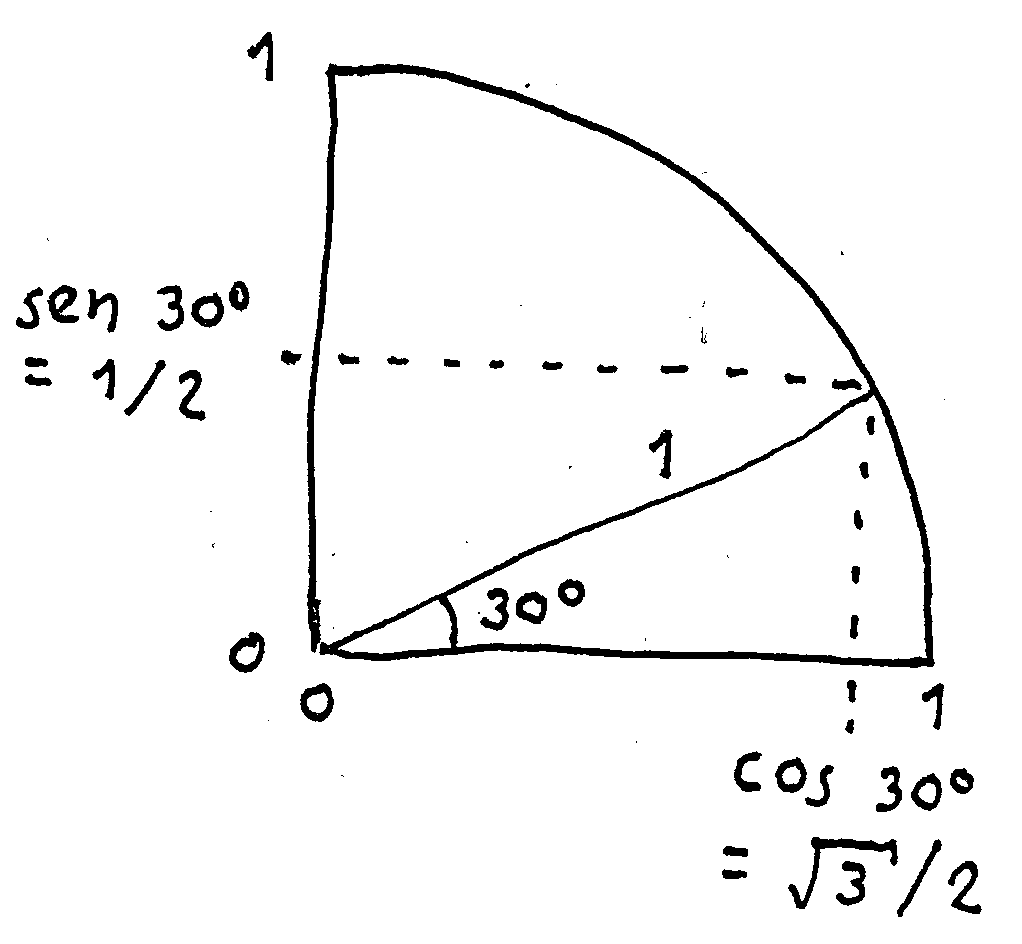
\includegraphics[height=3cm]{2021-1-C3/20210806_silvanus_triang_circ.pdf}
}
\quad
% (find-latexscan-links "C3" "20210806_silvanus_triang_1")
% (find-xpdf-page "~/LATEX/2021-1-C3/20210806_silvanus_triang_1.pdf")
\myvcenter{
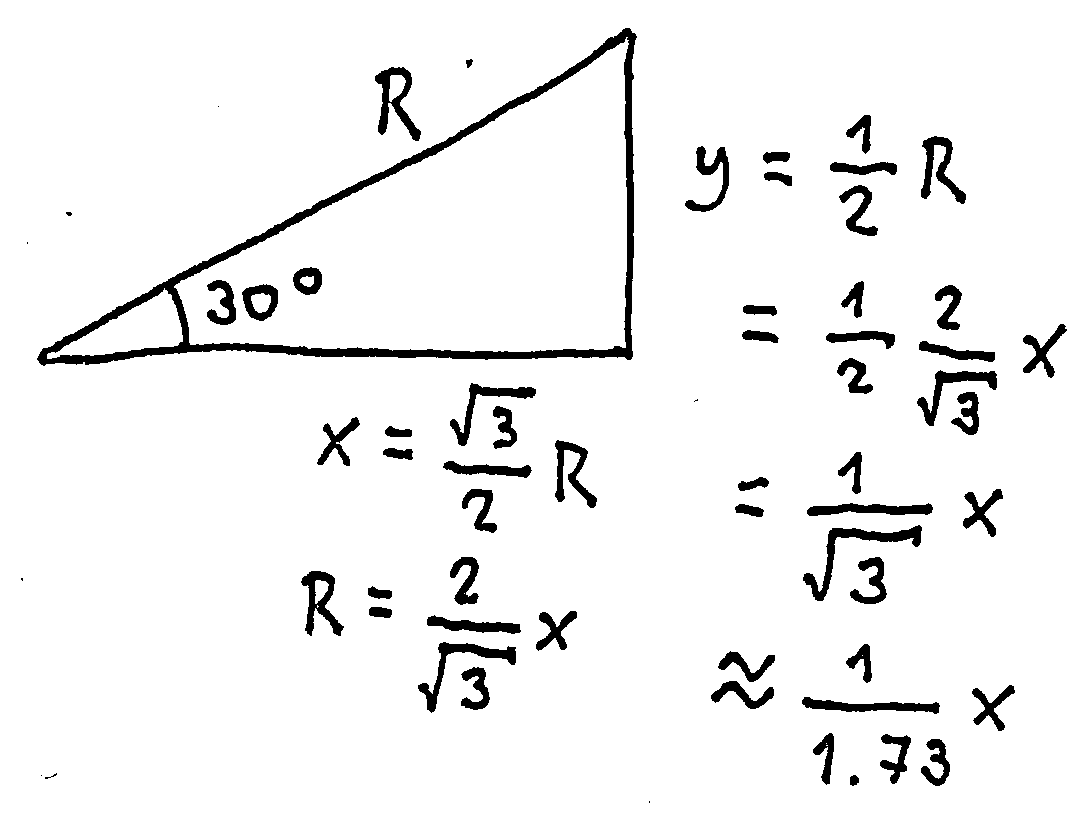
\includegraphics[height=3cm]{2021-1-C3/20210806_silvanus_triang_1.pdf}
}
\quad
% (find-latexscan-links "C3" "20210806_silvanus_triang_a_d")
% (find-xpdf-page "~/LATEX/2021-1-C3/20210806_silvanus_triang_a_d.pdf")
\myvcenter{
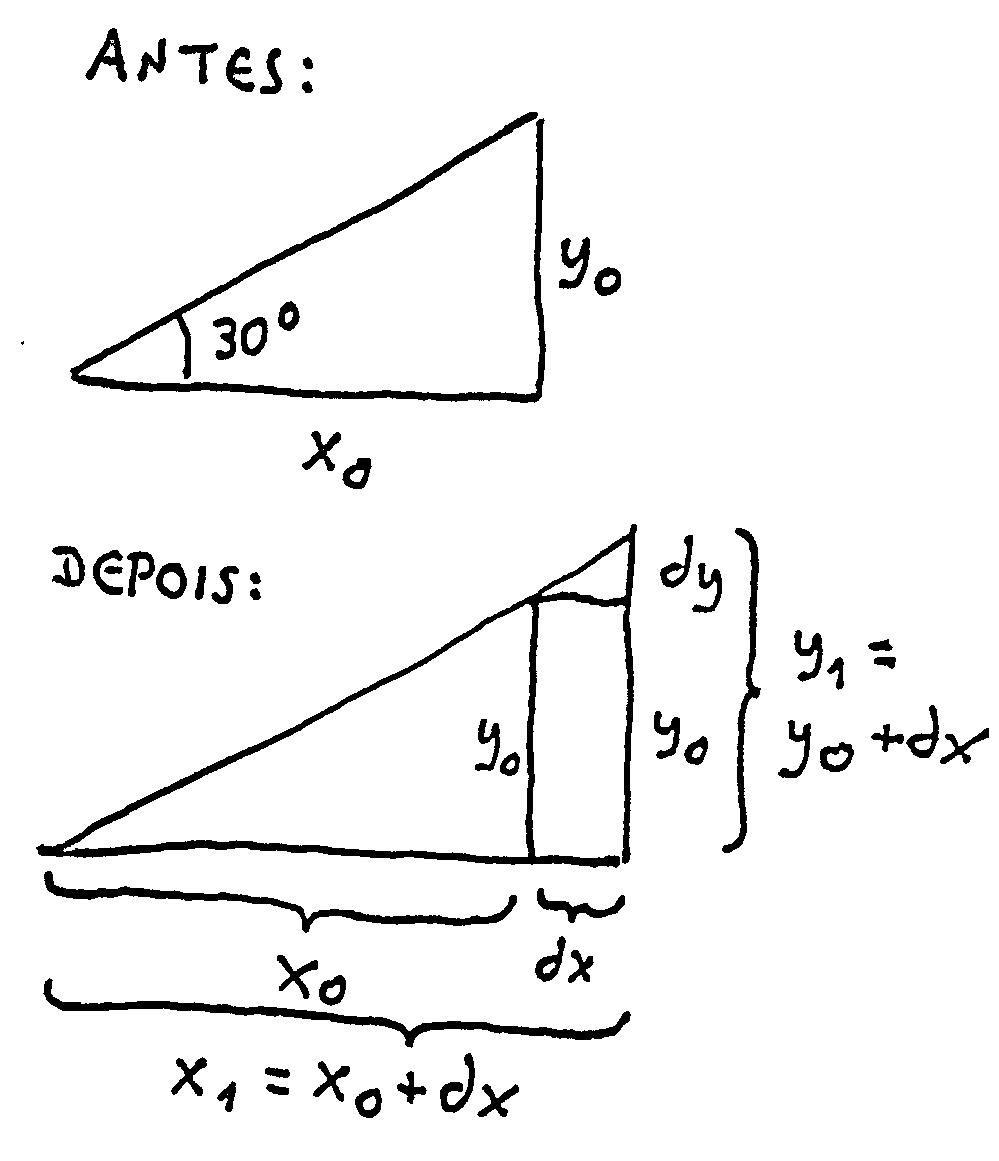
\includegraphics[height=4cm]{2021-1-C3/20210806_silvanus_triang_a_d.pdf}
}
$$

\newpage

%  _____                   _       
% | ____|___  ___ __ _  __| | __ _ 
% |  _| / __|/ __/ _` |/ _` |/ _` |
% | |___\__ \ (_| (_| | (_| | (_| |
% |_____|___/\___\__,_|\__,_|\__,_|
%                                  
% «silvanus-escada»  (to ".silvanus-escada")
% (c3m212nfp 14 "silvanus-escada")
% (c3m212nfa    "silvanus-escada")

{\bf Silvanus Thompson: o exemplo da escada (p.11)}


Links:

{\scriptsize

% (find-sthompsonpage (+ 11  11)   "ladder")
% (find-sthompsontext (+ 11  11)   "ladder")
% https://www.gutenberg.org/files/33283/33283-pdf.pdf#page=22
\url{https://www.gutenberg.org/files/33283/33283-pdf.pdf#page=22}

\url{http://angg.twu.net/eev-videos/2021-1-C3-notacao-de-fisicos-s-esc.mp4}

}

$$
% (find-latexscan-links "C3" "20210806_silvanus_escada_3d")
% (find-xpdf-page "~/LATEX/2021-1-C3/20210806_silvanus_escada_3d.pdf")
\myvcenter{
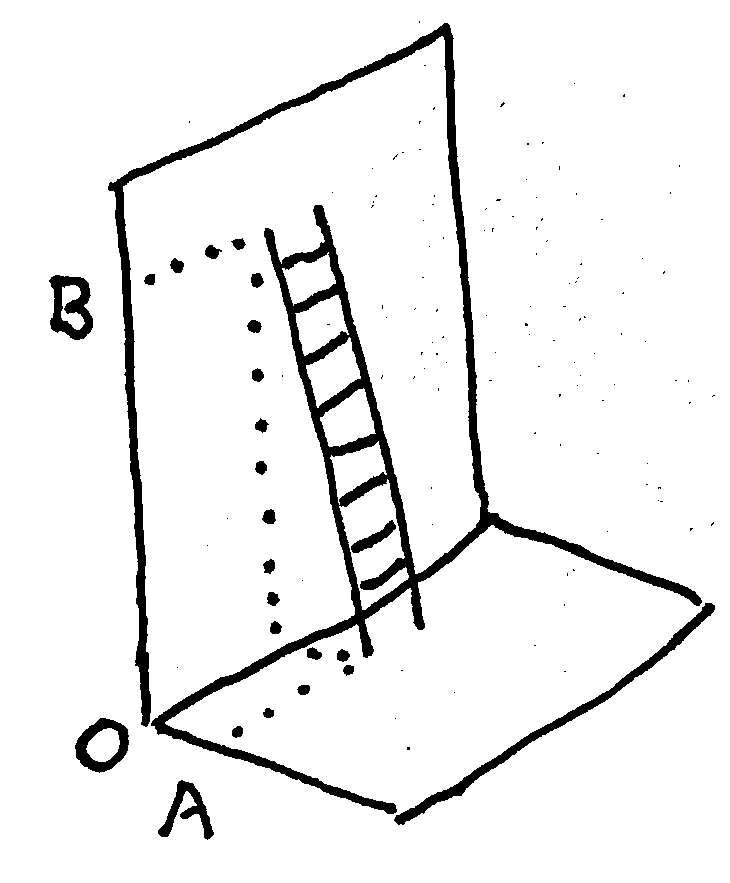
\includegraphics[height=3cm]{2021-1-C3/20210806_silvanus_escada_3d.pdf}
}
\quad
% (find-latexscan-links "C3" "20210806_silvanus_escada")
% (find-xpdf-page "~/LATEX/2021-1-C3/20210806_silvanus_escada.pdf")
\myvcenter{
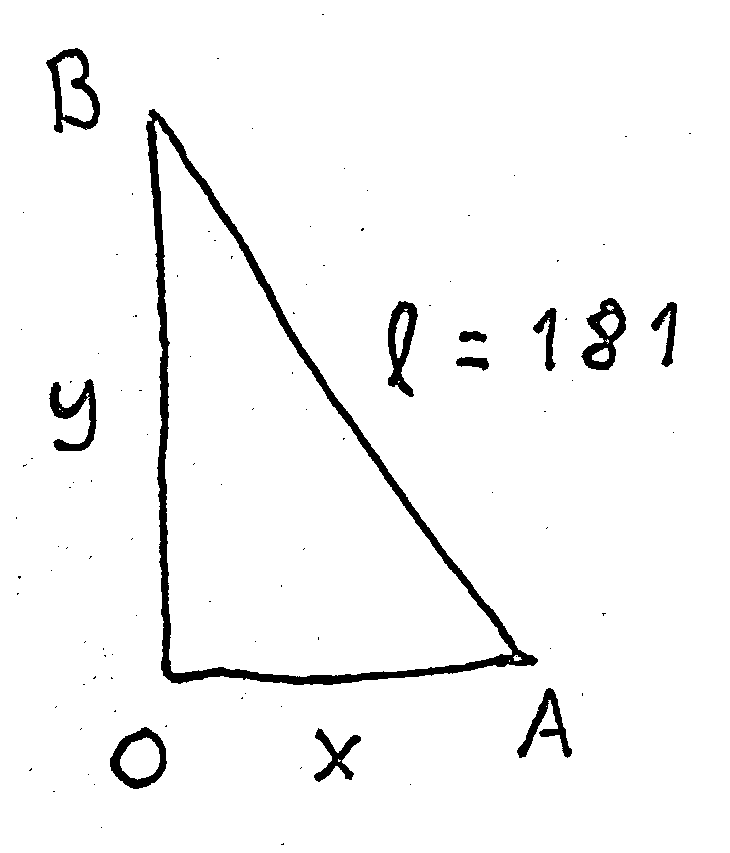
\includegraphics[height=3cm]{2021-1-C3/20210806_silvanus_escada.pdf}
}
\quad
% (find-latexscan-links "C3" "20210806_silvanus_escada_antes")
% (find-xpdf-page "~/LATEX/2021-1-C3/20210806_silvanus_escada_antes.pdf")
\myvcenter{
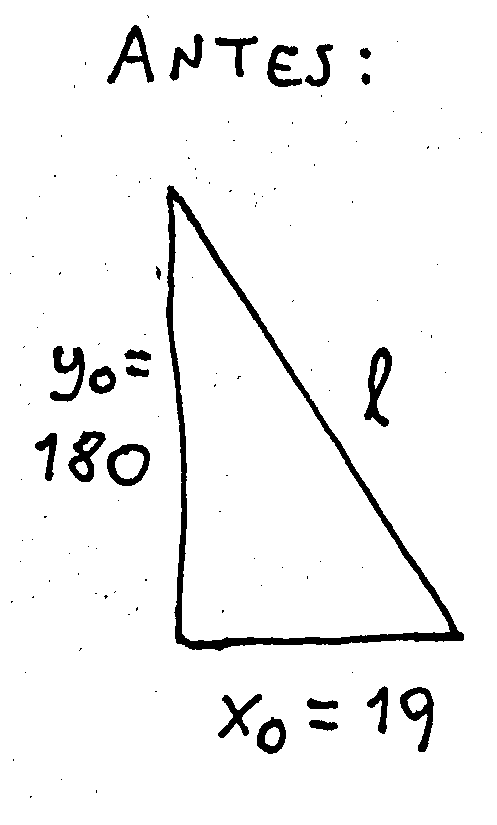
\includegraphics[height=3.2cm]{2021-1-C3/20210806_silvanus_escada_antes.pdf}
}
\quad
% (find-latexscan-links "C3" "20210806_silvanus_escada_depois")
% (find-xpdf-page "~/LATEX/2021-1-C3/20210806_silvanus_escada_depois.pdf")
\myvcenter{
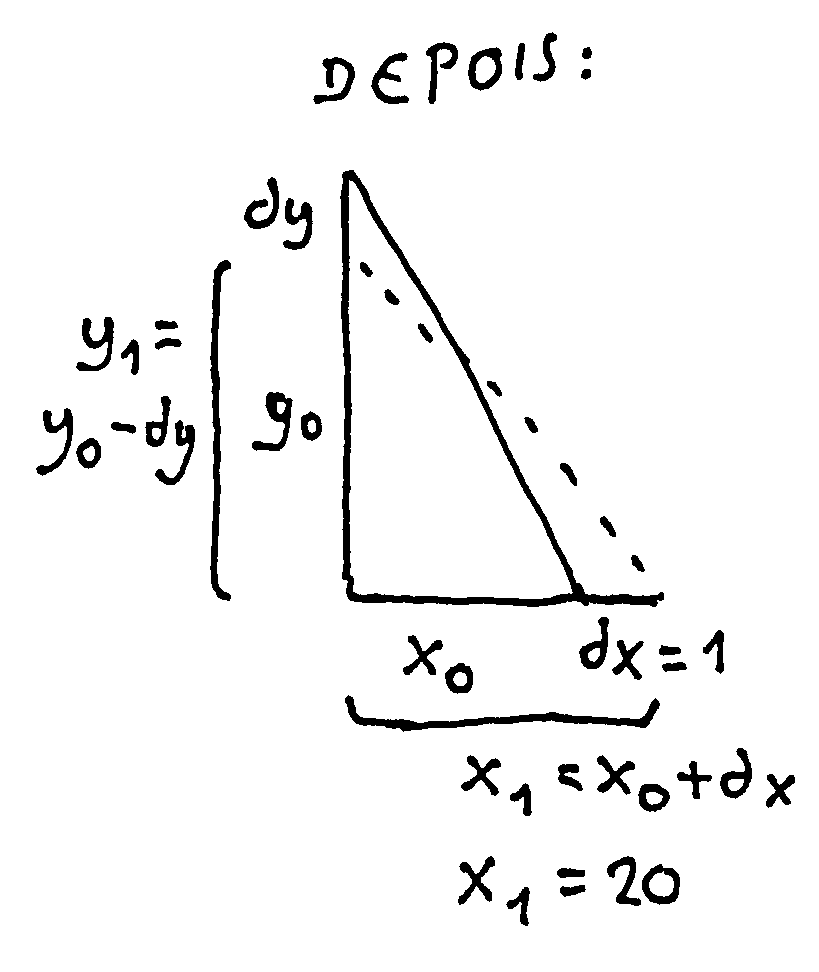
\includegraphics[height=4cm]{2021-1-C3/20210806_silvanus_escada_depois.pdf}
}
$$


\newpage

% «escada-contas»  	(to ".escada-contas")
% (c3m212nfp 15 "escada-contas")
% (c3m212nfa    "escada-contas")

{\bf Silvanus Thompson: o exemplo da escada: contas}

\msk

% (find-latexscan-links "C3" "20210806_silvanus_escada_contas")
% (find-xpdf-page "~/LATEX/2021-1-C3/20210806_silvanus_escada_contas.pdf")
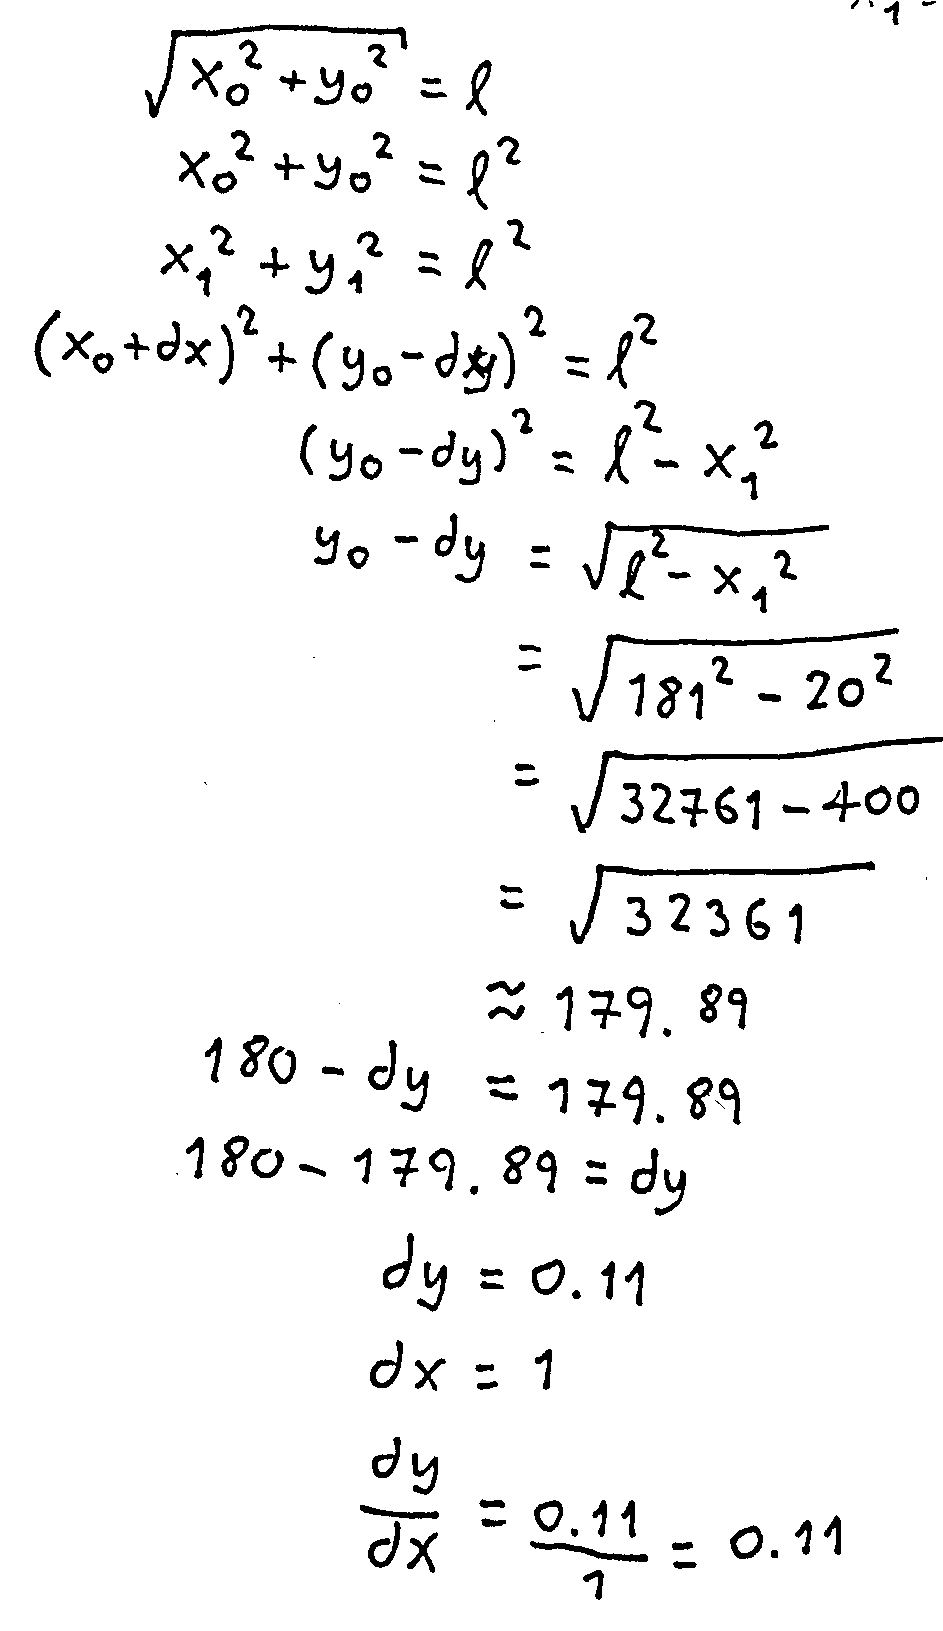
\includegraphics[height=7.0cm]{2021-1-C3/20210806_silvanus_escada_contas.pdf}

\newpage

% «exercicio-2»  (to ".exercicio-2")
% (c3m212nfp 16 "exercicio-2")
% (c3m212nfa    "exercicio-2")

{\bf Exercício 2}

% (find-books "__analysis/__analysis.el" "thompson")
% (find-sthompsonpage (+ 11  25) "V. Next Stage. What to do with Constants")

Nas páginas 25 e 26 o Thompson faz uma contas e conclui

que se $y = x^3+5$ então $\frac{dy}{dx} = 3x^2$. Entenda as contas dele

e traduza-as pra notação modernizada.

Link:

%  https://www.gutenberg.org/files/33283/33283-pdf.pdf#page=36
\u{https://www.gutenberg.org/files/33283/33283-pdf.pdf\#page=36}


\newpage

{\bf Exercício 2: dicas}

$$\begin{array}{rcl}
  y_0 &=& x_0^3+5 \\
  y_1 &=& x_1^3+5 \\
      &=& (x_0+Δx)^3+5 \\
  (x_0+Δx)^3 &=& x_0^3 + 3x_0^2Δx + 3x_0(Δx)^2 + (Δx)^3 \\
  \end{array}
$$

Tente simplificar $\frac{Δy}{Δx}$, leia o Thompson supondo que

$Δx$ é muito pequeno, e tente entender como ele lida

com termos que ele considera ``desprezíveis''.

\bsk

Mais uma idéia: quando $y=y(x)$

e $Δx$ é muito pequeno temos $\frac{dy}{dx}Δx ≈ Δy$.

O Thompson escreve isto como $\frac{dy}{dx}dx = dy$.


\newpage

% «exercicio-2-dicas-2»  (to ".exercicio-2-dicas-2")
% (c3m212nfp 17 "exercicio-2-dicas-2")
% (c3m212nfa    "exercicio-2-dicas-2")

{\bf Exercício 2: mais dicas}

Repare que você está tentando aprender três ``notações'' ao mesmo
tempo: a do livro do Thompson (``T''), a versão modernizada da notação
do Thompson (``M''), e a ``notação de matemáticos'' do livro do
Bortolossi (``B'')...

Se você tiver um procedimento pra traduzir, por exemplo, a notação T
pra notação B, você pode usá-lo pra aprender a fazer a tradução
oposta, de B pra T... você pode fazer uma tabela com expressões e
contas na primeira notação e as traduções delas pra segunda notação e
usar essa tabela pra tentar descobrir como a tradução da segunda
notação pra primeira deve funcionar.




\newpage

% «variaveis-novas»  (to ".variaveis-novas")
% (c3m212nfp 19 "variaveis-novas")
% (c3m212nfa    "variaveis-novas")

{\bf O truque das variáveis novas}

\scalebox{0.85}{\def\colwidth{12cm}\firstcol{

No capítulo 6 o Thompson calcula $\ddx((x^2 + c) + (ax^4 + b))$

organizando as contas mais ou menos desta forma:

$$\begin{array}{rcl}
  y &=& (x^2 + c) + (ax^4 + b) \\
  \frac{dy}{dx} &=& \frac{d((x^2+c) + (ax^4+b))}{dx} \\
                &=& \frac{d(x^2+c)}{dx} + \frac{d(ax^4+b)}{dx} \\
                &=& 2x + 4ax^3 \\
  \end{array}
$$

No capítulo 9 -- ``Introducing a useful dodge'' --

o Thompson mostra como a gente pode simplificar contas

como essa introduzindo ``variáveis dependentes'' novas.

\bsk

{\bf Exercício 3.}

Entenda os exemplos (1)--(4) das páginas 66--68 do Thompson.

\bsk

{\bf Exercício 4.}

Faça os exercícios (1)--(4) das páginas 66--68 do Thompson.

}}

\newpage

% «derivadas-parciais»  (to ".derivadas-parciais")
% (c3m212nfp 20 "derivadas-parciais")
% (c3m212nfa    "derivadas-parciais")

% (find-books "__analysis/__analysis.el" "bortolossi")
% (find-bortolossi5page (+ -161 162) "5. Derivadas parciais")
% (find-bortolossi5page (+ -162 168) "Mais ainda")
% (find-bortolossi5page (+ -162 177) "5.5. Exercícios")

{\bf Derivadas parciais}

Nós vamos aprender derivadas parciais começando por

como calcular derivadas parciais de funções simples.

A explicação do Bortolossi é mais fácil de entender

que a do Thompson mas o truque de introduzir

variáveis novas do Thompson vai ser incrivelmente útil.

\msk


Leia as páginas 168 e 169 do capítulo 5 do Bortolossi.

Comece do último parágrafo da 168 -- o que começa com

``Mais ainda''. Leia a página 169 toda.

\bsk

{\bf Exercício 5.}

Faça todos os itens do exercício 1 da página 177

do capítulo 5 do Bortolossi.


\newpage

% «derivadas-parciais-th»  (to ".derivadas-parciais-th")
% (c3m212nfp 21 "derivadas-parciais-th")
% (c3m212nfa    "derivadas-parciais-th")
% (find-books "__analysis/__analysis.el" "thompson")
% (find-sthompsonpage (+ 11 172) "XVI. Partial Differentiation")

{\bf Derivadas parciais no Thompson}

Leia o início do capítulo XVI do Thompson --

da página 172 até a 174.

Entenda os exemplos (1) até (3).

\msk

Obs: a maioria dos livros modernos usa

uma definição de ``derivada total'' que não é

totalmente compatível com a definição de

``diferencial total'' do Thompson...

Fique preparado!

\bsk

{\bf Exercício 6.}

Faça os exercícios (1)--(6) das páginas

177 e 178 do Thompson.





\newpage

% «derivadas-parciais-e-ts»  (to ".derivadas-parciais-e-ts")
% (c3m212nfp 22 "derivadas-parciais-e-ts")
% (c3m212nfa    "derivadas-parciais-e-ts")

{\bf Derivadas parciais e derivadas totais}

Digamos que $z = z(x,y)$ e $y = y(x)$.

\msk

Vamos começar com um caso bem concreto --- um que

eu usei em EDOs com variáveis separáveis em C2... link:
\ssk

{\footnotesize

% (c2m211edovsa "title")
% (c2m211edovsa "title" "Aula 25: EDOs com variáveis separáveis")
\url{http://angg.twu.net/LATEX/2020-2-C2-edovs.pdf}

}

\msk

O nosso caso bem concreto vai ser:

$z = z(x,y) = x^2 + y^2$,

$y = y(x) = \sqrt{1 - x^2}$.

quando nós \ColorRed{só} consideramos o $z = z(x,y) = x^2 + y^2$

as derivadas parciais de $z$ são $z_x = 2x$ e $z_y = 2y$,

mas quando \ColorRed{também} consideramos o $y = y(x) = \sqrt{1 - x^2}$

aí temos $z = z(x,y(x)) = x^2 + \sqrt{1-x^2}^2 = 1$, e $\frac{dz}{dx}=0$.

\msk

Esta derivada $\frac{dz}{dx} = \frac{d}{dx} z(x,y(x))$ é chamada de

\ColorRed{derivada total} de $z$ com relação a $y$.




\newpage

% «exercicio-7»  (to ".exercicio-7")
% (c3m212nfp 23 "exercicio-7")
% (c3m212nfa    "exercicio-7")

{\bf Exercício 7.}

Digamos que $z = z(x,y) = (x+2)(y+3)$

e que $y = y(x) = \sen x$.

a) Calcule $\frac{∂z}{∂x}$, $\frac{∂z}{∂y}$.

b) Calcule $\frac{dz}{dx}$.

c) Calcule $\frac{d}{dx}\frac{d}{dx}z$.

\msk

\ColorRed{Convenção:} quando uma expressão como $z_x$ puder

ser interpretada tanto como uma derivada parcial quanto

como uma derivada total o default é interpretá-la

como derivada parcial.


\newpage

% «exercicio-8»  (to ".exercicio-8")
% (c3m212nfp 24 "exercicio-8")
% (c3m212nfa    "exercicio-8")

{\bf Exercício 8.}

Digamos que $z=z(x,y)$ e $y=y(x)$.

(Isto é uma versão mais geral do exercício 7).

\ssk

a) Calcule $\frac{d}{dx}z$.

\ssk

b) Calcule $\frac{d}{dx}\frac{d}{dx}z$.




\newpage






Tudo que vem depois daqui vai ser reescrito.




\newpage

% «quadraticas-exemplos»  (to ".quadraticas-exemplos")
% (c3m211nfp 18 "quadraticas-exemplos")
% (c3m211nfa    "quadraticas-exemplos")
% (c3m211qp 2 "figuras-3D")
% (c3m211qa   "figuras-3D")

{\bf Quadratics - tests}


% (c3m211cnp 3 "exercicio-1")
% (c3m211cna   "exercicio-1")

% (find-LATEX "2021-1-C3-3D.lua" "QuadraticFunction-tests")
%L
%L V3.__index.p1 = V{2, -0.5}
%L V3.__index.p2 = V{1,  1.5}
%L V3.__index.p3 = V{0,  2}
%L
%L V3.__index.p1 = V{2,   -0.5}
%L V3.__index.p2 = V{0.5, 1.7}
%L V3.__index.p3 = V{0,   0.5}

%L qf = QuadraticFunction {x0=3, y0=2, a=2, Dx=0, Dy=0, Dxx=0, Dyy=0, Dxy=1}
%L srf = Surface.new(qf, 3, 2)
\pu

\def\QuadraticInPerspective#1{
   \beginpicture(0,-3)(10,6)
     \pictgray{\expr{v3():xygrid(4,3)          }}
     \expr          {v3():axeswithticks(4,3,3) }
     \expr          {#1:diagonals(8, "c")      }
     \expr          {#1:square   (8, "0")      }
     \pictgray{\expr{#1:square   (2, "p")      }}
     \expr          {#1:square   (8, "c")      }
   \end{picture}}

$$\unitlength=10pt
  \QuadraticInPerspective{srf}
$$


\newpage

%L qf = QuadraticFunction {x0=3, y0=2, a=2, Dx=0, Dy=0, Dxx=1, Dyy=1, Dxy=0}
%L srf = Surface.new(qf, 3, 2)
\pu

$$\unitlength=10pt
  \QuadraticInPerspective{srf}
$$


\newpage

%L qf = QuadraticFunction {x0=3, y0=2, a=2, Dx=0, Dy=0, Dxx=1, Dyy=-1, Dxy=0}
%L srf = Surface.new(qf, 3, 2)
\pu

$$\unitlength=10pt
  \QuadraticInPerspective{srf}
$$


\newpage

% (c3m202planotangp 27 "3D-fig")
% (c3m202planotanga    "3D-fig")

% (find-LATEX "edrxgac2.tex" "beginpicture")

%L rv = savevars(function (...)
%L      ex,ey,vx,vy, A0, A,B,C,D,E,F,E,G = ... end,
%L      ex,ey,vx,vy, A0, A,B,C,D,E,F,E,G)
%L
%L ex = v3(1,0,0)
%L ey = v3(0,1,0)
%L vx = v3(0,0,0.5)
%L vy = v3(0,0,1.5)
%L vz = v3(0,0,0.5)
%L A0 = v3(2,1,0); B0 = A0 + ex; C0 = A0 + ey; D0 = B0 + ey
%L A  = A0 + vz
%L B  = A + ex
%L C  = A + ey
%L D  = A + ex + ey
%L E  = B + vx
%L F  = E + ey
%L G  = C + vy
%L H  = G + ex
%L I  = H + vx
%L
%L V3.__index.p1 = V{2, -0.5}
%L V3.__index.p2 = V{1,  1.25}
%L V3.__index.p3 = V{0,  2}
%L
\pu

$\vcenter{\hbox{%
 \unitlength=20pt
 \beginpicture(0,-4)(8,8)
%P \pictgray{<v3():xygrid(3,3)>}
%P <v3():axeswithticks(3,3,3)>
%P \pictgray{\Line<A0><A> \Line<B0><B> \Line<C0><C> \Line<D0><D>}
%P \Line<A><B><D><C><A>
%P \Line<A><E><B> \Line<E><F><I><E>
%P \Line<A><G><C> \Line<G><H><I><G>
%P \Line<D><F>
 \pu
 \end{picture}%
 }}
$
%

%L rv()
\pu


\newpage

% «thomas»  (to ".thomas")
% (find-books "__analysis/__analysis.el" "thomas")
% (find-thomas11-1page (+  25  159) "3.2" "Differentiation rules")
% (find-thomas11-1page (+  26  171) "3.3" "The derivative as a rate of change")
% (find-thomas11-1page (+  28  183) "3.4" "Derivatives of trigonometric functions")
% (find-thomas11-1page (+  30  190) "3.5" "The chain rule and parametric equations")
% (find-thomas11-1page (+  32  205) "3.6" "Implicit differentiation")
% (find-thomas11-1page (+  34  213) "3.7 Related Rates")
% (find-thomas11-1page (+  35  221) "3.8 Linearization and Differentials")

% «bortolossi»  (to ".bortolossi")
% (find-bortolossi7page (+ -238 256)    "matriz jacobiana")
% (find-bortolossi7page (+ -238 261)    "Teorema 7.6")
% (find-bortolossi7page (+ -238 263) "7.3. Composição de funções")
% (find-bortolossi7page (+ -238 266) "7.5. A regra da cadeia em Cálculo 2")
% (find-bortolossi7page (+ -238 266)    "Teorema 7.7")

% «segundo-exemplo»  (to ".segundo-exemplo")
% (c3m211nfp 6 "segundo-exemplo")
% (c3m211nfa   "segundo-exemplo")

{\bf Um segundo exemplo}

Digamos que o conjunto dos pontos $(x,y)$

``que obedecem as restrições'' é esse aqui:
%
$$\setofst{(x,y)∈\R^2}{x^2+y^2=5}$$

e que $(x_0,y_0) = (3,4)$.

\bsk
\bsk

Os físicos consideram que ``é óbvio'' que (em geral!) variáveis

``variam continuamente'', então se $x_1=x_0+Δx$ e $y_1=y_0+Δy$

e $Δx$ é muito pequeno então $Δy$ é muito pequeno também.

(Veja o vídeo!...)




% O meu modo preferido de formalizar a notação de físicos é esse aqui.

% Silvanus P. Thompson:
% (find-books "__analysis/__analysis.el" "silvanus")
% (find-books "__analysis/__analysis.el" "kelley" "complete_idiots_guide")
% https://calculusmadeeasy.org/2.html negligible
% https://calculusmadeeasy.org/16.html



%\printbibliography

\GenericWarning{Success:}{Success!!!}  % Used by `M-x cv'

\end{document}

%  ____  _             _         
% |  _ \(_)_   ___   _(_)_______ 
% | | | | \ \ / / | | | |_  / _ \
% | |_| | |\ V /| |_| | |/ /  __/
% |____// | \_/  \__,_|_/___\___|
%     |__/                       
%
% «djvuize»  (to ".djvuize")
% (find-LATEXgrep "grep --color -nH --null -e djvuize 2020-1*.tex")

 (eepitch-shell)
 (eepitch-kill)
 (eepitch-shell)
# (find-fline "~/2021.2-C3/")
# (find-fline "~/LATEX/2021-2-C3/")
# (find-fline "~/bin/djvuize")

cd /tmp/
for i in *.jpg; do echo f $(basename $i .jpg); done

f () { rm -v $1.pdf;  textcleaner -f 50 -o  5 $1.jpg $1.png; djvuize $1.pdf; xpdf $1.pdf }
f () { rm -v $1.pdf;  textcleaner -f 50 -o 10 $1.jpg $1.png; djvuize $1.pdf; xpdf $1.pdf }
f () { rm -v $1.pdf;  textcleaner -f 50 -o 20 $1.jpg $1.png; djvuize $1.pdf; xpdf $1.pdf }

f () { rm -fv $1.png $1.pdf; djvuize $1.pdf }
f () { rm -fv $1.png $1.pdf; djvuize WHITEBOARDOPTS="-m 1.0 -f 15" $1.pdf; xpdf $1.pdf }
f () { rm -fv $1.png $1.pdf; djvuize WHITEBOARDOPTS="-m 1.0 -f 30" $1.pdf; xpdf $1.pdf }
f () { rm -fv $1.png $1.pdf; djvuize WHITEBOARDOPTS="-m 1.0 -f 45" $1.pdf; xpdf $1.pdf }
f () { rm -fv $1.png $1.pdf; djvuize WHITEBOARDOPTS="-m 0.5" $1.pdf; xpdf $1.pdf }
f () { rm -fv $1.png $1.pdf; djvuize WHITEBOARDOPTS="-m 0.25" $1.pdf; xpdf $1.pdf }
f () { cp -fv $1.png $1.pdf       ~/2021.2-C3/
       cp -fv        $1.pdf ~/LATEX/2021-2-C3/
       cat <<%%%
% (find-latexscan-links "C3" "$1")
%%%
}

f 20201213_area_em_funcao_de_theta
f 20201213_area_em_funcao_de_x
f 20201213_area_fatias_pizza



%  __  __       _        
% |  \/  | __ _| | _____ 
% | |\/| |/ _` | |/ / _ \
% | |  | | (_| |   <  __/
% |_|  |_|\__,_|_|\_\___|
%                        
% <make>

 (eepitch-shell)
 (eepitch-kill)
 (eepitch-shell)
# (find-LATEXfile "2019planar-has-1.mk")
make -f 2019.mk STEM=2021-2-C3-notacao-de-fisicos veryclean
make -f 2019.mk STEM=2021-2-C3-notacao-de-fisicos pdf

% Local Variables:
% coding: utf-8-unix
% ee-tla: "c3nf"
% ee-tla: "c3m212nf"
% End:
